\chapter{Nawigacja robotów w obecności ludzi}

Problem nawigacji robotów w środowisku człowieka, znany w literaturze anglojęzycznej jako {\textit{human-aware navigation}}, jest zagadnieniem badawczym o rosnącej popularności. W trakcie badań określono następujące problemy odnoszące się do ruchu robota\cite{survey}:

\begin{itemize}
\item Bezpieczeństwo ludzi i robota
\item Komfort ludzi, czyli brak stresu wywołanego nieprawidłowym zachowaniem robota
\item Naturalność, a więc podobieństwo zachowania robota do ludzkiego
\item Zdolność robota do rozumienia i imitacji konwencji kulturowych.
\end{itemize}

Zauważono również, że kwestia bezpieczeństwa ruchu nie jest tożsama z komfortem ludzi, gdyż robot może poruszać się bezpiecznie, nie doprowadzać do kolizji z człowiekiem, lecz dla człowieka jego zachowanie może wydawać się niepewne, nie wzbudzać zaufania ludzi do użytej technologii \cite{survey}. \\

\indent Podstawą do rozważań jest studium E. T. Halla na temat dystansu interpersonalnego \cite{dimension}, które wyróżnia cztery strefy:

\begin{itemize}
\item strefa intymna - strefa bliskich relacji, dotyk - do 0.5m
\item strefa personalna - interakcje w obrębie przyjaciół i rodziny - od 0.5m do 1.2m
\item strefa społeczna - interakcje ze znajomymi - od 1.2m od 3.7m
\item - strefa publiczna - publiczne wystąpienia - od 3.7m.
\end{itemize}

\begin{figure}[H]
	\centering
	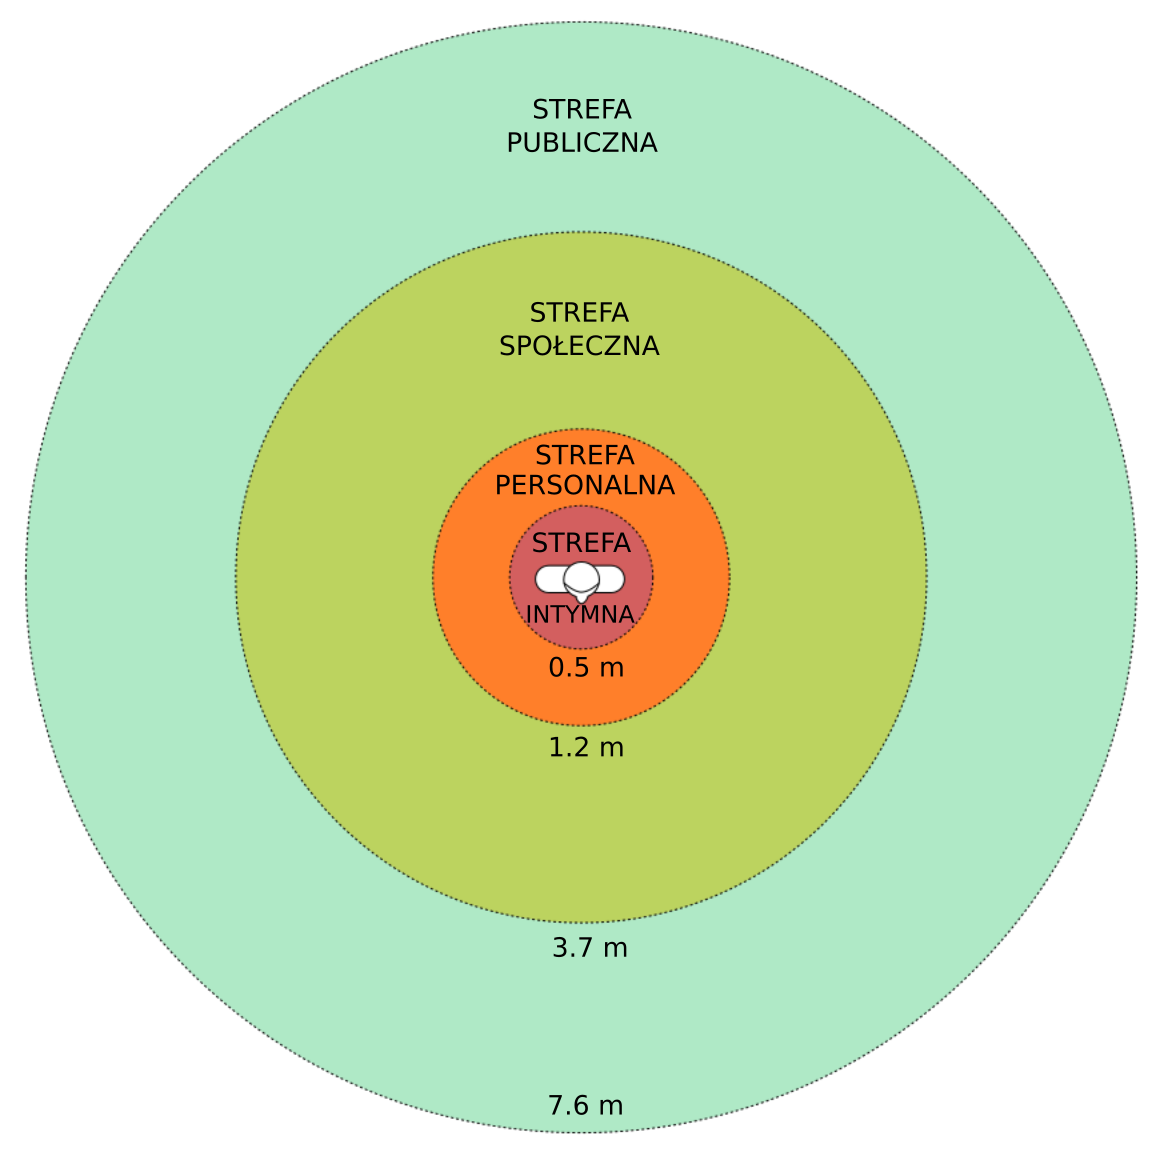
\includegraphics[width=0.6\textwidth]{gfx/882px-Personal_Spacepl.png}
	\caption{Przedstawienie stref zaproponowanych przez E.T. Halla w metrach, na bazie rysunku \cite{dimension_zones}}
	\label{fig:hall_zones}
\end{figure}

\indent Badania dotyczące stref społecznych mają istotne znaczenie dla określenia naturalności ruchu robota. Robot pracujący z człowiekiem musi zachować odległości, zależnie od wykonywanych zadań i konstrukcji robota. Strefy personalne implementowane najczęściej za pomocą pól potencjału, bądź funkcji kosztu \cite{survey}. Drugie podejście obrazuje rysunek [\ref{fig:cost_zones}]. Podobną koncepcję można również wykorzystać w przypadku poruszającego się człowieka, gdzie kształt strefy personalnej, na bazie wektora ruchu, można obliczyć za pomocą funkcji gaussowskich\cite{nrs} \cite{gauss_2}. Część badaczy wysuwa jednak wniosek, że istotniejszym czynnikiem niż zachowanie odległości, jest przestrzeganie zasad społecznych, kulturowych. To ich naruszenie powoduje dyskomfort pracy z robotem \cite{survey},\cite{survey_2}. Pożądaną umiejętnością robota jest także zmniejszeniee prędkości przy podejściu do człowieka, oraz zachowanie odpowiedniego kierunku skierowania czujników, dla robotów przypominająych istoty humanoidalne.

\begin{figure}[H]
	\centering
	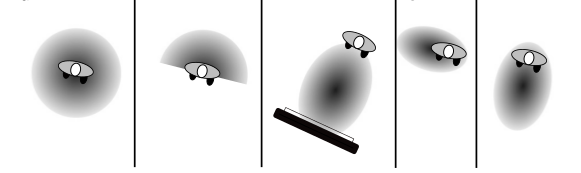
\includegraphics[width=0.75\textwidth]{gfx/cost_zone.png}
	\caption{Przykładowe strefy o zwiększonym koszcie ruchu wokół człowieka. Mogą się one różnić w zależności od przyjętych założeń\cite{survey}. $a)$ strefa o kształcie symetrycznym, kołowym, $b)$ strefa o kształcie półkola - robot może poruszać się tuż przed twarzą osoby, lecz nie tuż za jej plecami, $c)$, $d)$ strefa eliptyczna skierowana zgodnie z orientacją osoby, $d)$ strefa eliptyczna zwrócona w kierunku prawej strony osoby - robot będzie preferował ruch z jej lewej strony }
	\label{fig:cost_zones}
\end{figure}

Kwestia nawigacji i unikania kolizji robot-człowiek nie byłaby możliwa bez rozwiązania problemu planowania ścieżki ruchu. Jedną z możliwych klasyfikacji metod planowania ścieżek ruchu przestawia rysunek [\ref{fig:taxonomy}].

\begin{figure}[H]
	\centering
	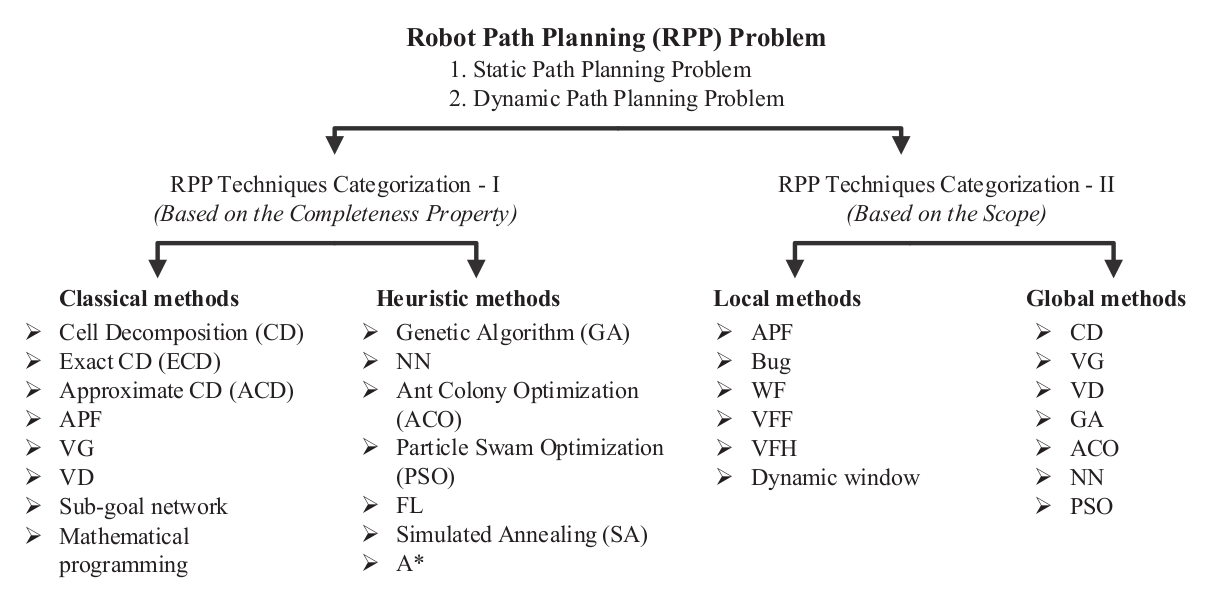
\includegraphics[width=0.9\textwidth]{gfx/taksonomia_planery.png}
	\caption{Taksonomia algorytmów planowania ścieżki dla robotów mobilnych\cite{taxonomy}}
	\label{fig:taxonomy}
\end{figure}


\indent Algorytmy planowania ścieżki można podzielić na metody statyczne i dynamiczne. Metody statyczne zakładają, informację na temat środowiska znane są a priori, a środowisko jest niezmienne. Metody dynamiczne nie posiadają z góry zdefioniowanego środowiska, bądź jest ono zdefiniowane jedynie częściowo. Algorytmy można również podzielić ze względu na $kompletność$ i $zasięg$. Kompletność określa czy w przypadku istienia ścieżki ruchu, zostanie ona z pewnością znaleziona przez algorytm. Wyróżniamy metody klasyczne i heurystyczne. Celem metod klasycznych jest wyznacznie najlepszej dopuszczalnej ścieżki ruchu, bądź stwierdzenie, że takowa nie istnieje. Odbywa się to jednak kosztem dużego nakładu obliczeniowego. Algorytmy heurystyczne nie gwarantują znalezienia optymalnego rozwiązania, ani znalezienia rozwiązania, nawet jeśli takowe istnieje \cite{planer_1}. Zaletą algorytmów heurystycznych jest jednak większa szybkość działania. Ze względu na zasięg, algorytmy można podzielić również na metody globalne i lokalne. Metody globalne umożliwiają znalezienie całej ścieżki ruchu przed jego rozpoczęciem. W metodach globalnych zakłada się dostępność modelu środowiska. Nie są one jednak efektywne w przypadku dynamicznych przeszkód. Do tego celu wykorzystuje się metody lokalne, które operują na danych dostarczonych przez czujniki, takie jak kamery RGB czy skanery laserowe \cite{taxonomy},\cite{planer_1},\cite{planer_2}. Metody lokalne planują ścieżkę ruchu inkrementacyjnie, istnieje jednak możliwość niepowodzenia generacji ścieżki. Często więc systemy planowania ścieżki ruchu budowane są z użyciem dwóch planistów, globalnego, który wyznacza ogólną ścieżkę ruchu od robota do zadanego celu i lokalnego, którego zadaniem jest obliczenie aktualnego wycinka ścieżki \cite{taxonomy}. \\
\indent Popularnym podejściem stosowanym przy implementacji planisty lokalnego jest Metoda Okna Dynamicznego (Dynamic Window Approach). W metodzie uwzględnia się wszystkie ograniczenia ruchu robota i w każdej iteracji tworzy zadaną liczbę par $(v,w)$, będących parami prędkościami liniowymi i kątowymi robota. Następnie dla każdej pary badany jest wpływ jej zastosowania na przyszły stan robota - to czy zderzy się on z przeszkodą, czy podąży w stronę celu, czy będzie trzymał się zadanej globalnej ścieżki itp. \cite{dwa}. Wszystkie możliwe trajektorie są oceniane i wybierana jest najwyżej punktowana. Sposób oceny można dostosować zmieniając wagi kryteriów.\\
\indent Kompletnym systemem realizującym zadania nawigacji w środowisku człowieka jest system opracowany przez Sisbota i.in. w 2007, opisany w pracy \cite{ma}. Praca zakładała stworzenie systemu planowania ruchu uwzględniającego pozycje, posturę (siedząca, stojąca) oraz zależności przestrzennych, takie jak nie przejeżdzanie w niewielkiej odległości od człowieka, tuż za jego plecami, czy też bliskość przeszkód blokujących pole widzenia danej osoby. 

Niezależnie od modułu planowania ścieżki ruchu zaimplementowano również system wykrywania człowieka na bazie odczytów czujników laserowych oraz kamery RGB. Dane pozyskane z sensorów laserowych były przetwarzane przez algorytm pozwalający na wykrycie nóg człowieka. Na tej podstawie można było stwierdzieć jego położenie. Obraz z kamery RGB służył do detekcji twarzy z bliskiej odległości.
\indent Badacze sformułowali dwa kryteria: bezpieczeństwa - zapewniające bezpieczeństwo człowiekowi i robotowi, poprzez zapewnienie odpowiedniego odległości oraz widoczności - stwierdzono, że ludzie czują się lepiej, gdy robot znajduję się możliwie długo w ich polu widzenia. Koszt łączny bezpieczeństwa i widoczności \eqref{eq:cost_1}, był następnie nanoszony na mapę kosztu, z której korzystał zaimplementowany planista ruchu nazwany HAMP (Human Aware Motion Planer).

\begin{figure}[h!t]
  	\centering 
  	\begin{equation} \label{eq:cost_1}
  	Cost_{merged}(x,y) = w_{1}Cost_{safety}(x,y) + w_{2}Cost_{visibility}(x,y)
  	\end{equation}   
  	\capequation{gdzie $x$ i $y$ to współrzędne na mapie, a $w_{1}$ i $w_{2}$ to współczynniki wagowe.} 
\end{figure}

A. Mateus w pracy \cite{nrs} przedstawia implementację systemu wykorzystującego moduł nawigacyjny ($navigation$) wbudowany w środowisko ROS. Celem systemu było wykrycie człowieka i planowanie ścieżki ruchu uwzględniającej szereg ograniczeń, m.in. odległość od człowieka, jak najniższy koszt zaplanowanej trasy, nawigacja ze stałą prędkością, czy omijanie ludzi z ich lewej strony. System zakładał istnieje globalnego i lokalnego modułu planowania ścieżki. Globalny wykorzystywał algorytm $A^*$ (rozważany był również algorytm Dijkstry), a lokalny algorytm $Trajectory$ $Rollout$. Model środowiska budowano za pomocą pakietu $costmap\_2d$, będącym częścią środowiska ROS. Zawiera on implementacje map kosztów. Wykryte osoby były na nie nanoszone wykorzystując zdefiniowaną przez autora fukcję gaussa. W innej pracy \cite{gauss_2} D. Vasquez i.in. proponują system zawierający wykrywanie i śledzenie ludzi, predykcje konfiguracji otoczenia, biorąc pod uwagę pozycję i prędkość ludzi, oraz nawigację robota. System predykcyjny skonstruowany został za pomocą Rosnącego Ukrytego Modelu Markova \cite{markov} oraz Filtru Kalmana. Strefa personalna człowieka modelowana była ponownie z wykorzystaniem funkcji gaussa. R. Kirby w pracy \cite{survey_3} przestawia strukturę strukturę systemu nawigacyjnego akceptowalnego przez ludzi z użyciem metody zoptymalizowanej pod kątem ograniczeń ruchu ($Constraint-Optimizing$
$Method$ $for$ $Person–Acceptable$ $NavigatION$ $- COMPANION$). Praca rozwija temat ograniczeń ruchu robota w środowisku pracy z ludźmi, planowania ścieżki oraz śledzenia (wizyjnego) ludzi, oraz podążania za nimi. Wśród zdefioniowanych ograniczeń ruchu występują: minimalny dystans robota od człowieka, odpowiednia przestrzeń buforowa pomiędzy przeszkodami a robotem, przestrzeganie stref komfortu człowieka, omijanie człowieka z prawej jego strony oraz poruszanie się robota zgodnie z kierunkiem zwrotu jego "twarzy". W systemie zaproponowano użycie robota opartego o platformę dookólną.
    
    
